\documentclass[11pt,letterpaper]{article}
\usepackage[lmargin=1in,rmargin=1in,tmargin=1in,bmargin=1in]{geometry}

% -------------------
% Packages
% -------------------
\usepackage{
	amsmath,			% Math Environments
	amssymb,			% Extended Symbols
	enumerate,		    % Enumerate Environments
	graphicx,			% Include Images
	lastpage,			% Reference Lastpage
	multicol,			% Use Multi-columns
	multirow			% Use Multi-rows
}
\graphicspath{ {./Images/} }


% -------------------
% Font
% -------------------
\usepackage[T1]{fontenc}
\usepackage{charter}


% -------------------
% Heading Commands
% -------------------
\newcommand{\class}{EECS 16ML}
\newcommand{\term}{Fall 2020}
\newcommand{\instructor}{Team RAAAK}
\newcommand{\head}[2]{%
\thispagestyle{empty}
\vspace*{-0.5in}
\noindent\begin{tabular*}{\textwidth}{l @{\extracolsep{\fill}} r @{\extracolsep{6pt}} l}
	\textbf{Quiz Topic: Outlier Removal via OMP} \\
	\textbf{\class:\; \term} & & \\
	\textbf{\instructor}
\end{tabular*} \\
\rule[2ex]{\textwidth}{2pt} %
}


% -------------------
% Commands
% -------------------
\newcommand{\prob}{\noindent\textbf{Problem. }}
\newcounter{problem}
\newcommand{\problem}{
	\stepcounter{problem}%
	\noindent \textbf{Part \theproblem. }%
}
\newcommand{\pointproblem}[1]{
	\stepcounter{problem}%
	\noindent \textbf{Problem \theproblem.} (#1 points)\,%
}
\newcommand{\pspace}{\par\vspace{\baselineskip}}
\newcommand{\ds}{\displaystyle}


% -------------------
% Header & Footer
% -------------------
\usepackage{fancyhdr}

\fancypagestyle{pages}{
	%Headers
	\fancyhead[L]{}
	\fancyhead[C]{}
	\fancyhead[R]{}
\renewcommand{\headrulewidth}{0pt}
	%Footers
	\fancyfoot[L]{}
	\fancyfoot[C]{}
	\fancyfoot[R]{}
\renewcommand{\footrulewidth}{0.0pt}
}
\headheight=0pt
\footskip=14pt

\pagestyle{pages}


% -------------------
% Content
% -------------------
\begin{document}
\textbf{EECS 16ML Quiz: Outlier Removal via OMP} \pspace


% Question 1
\problem Use the following matrix equation setup to run OMP for two iterations. Please box the intermediate and final residuals as well as the two components identified to have non-zero entries.

\begin{equation*}
    \begin{bmatrix}
        \boldsymbol{A} & \boldsymbol{I}
    \end{bmatrix}\begin{bmatrix}
        \vec{x} \\
        \vec{\epsilon}
    \end{bmatrix}
     = \vec{y} \Rightarrow
    \begin{bmatrix}
         1 & 1 & 0 & 1 & 1 & 0 & 0 & 0 \\
         1 & 1 & 0 & 0 & 0 & 1 & 0 & 0 \\
         1 & 0 & 1 & 1 & 0 & 0 & 1 & 0 \\
         1 & 0 & 1 & 0 & 0 & 0 & 0 & 1
    \end{bmatrix}
    \begin{bmatrix}
         a \\ b \\ c \\ d \\ e \\ f \\ g \\ h
    \end{bmatrix}
    =\begin{bmatrix}
         2 \\ 0 \\ 2 \\ 1
    \end{bmatrix}
\end{equation*}

\begin{enumerate}
    \item Iteration 1 Component: \vspace{3cm}
	\item Iteration 1 Residual: \vspace{3cm}
	\item Iteration 2 Component: \vspace{3cm}
	\item Iteration 2 Residual: \vspace{3cm}
\end{enumerate} 

\newpage
% Question 2
\problem Ignore the calculations done in the first problem. Suppose that a genie ran OMP for the problem above and told you the following about the sparse solution: %\vfill
\begin{equation*}
    \vec{x} = \begin{bmatrix}
        \frac{1}{2} \\ 1 \\ -\frac{1}{2} \\ 1
    \end{bmatrix}, \vec{\epsilon} = \begin{bmatrix}
        0 \\ 10 \\ -\frac{1}{2} \\ 0
    \end{bmatrix}
\end{equation*}
Interpret the results by identifying the outlier(s). Provide justification/explanation.
\vspace{5cm}


% Question 3
\problem In each of the three parts below, describe a potential stopping condition discussed in this course for OMP. In addition to naming the stopping condition, describe potential (dis)advantages and/or use cases. The order you list them in does not matter.
	\begin{enumerate}
	\item Stopping Condition 1: 
	    \begin{enumerate}[(a)]
	        \item Description:\vspace{1cm}
	        \item Use Cases: \vspace{1cm}
	    \end{enumerate}
	\item Stopping Condition 2: 
	    \begin{enumerate}[(a)]
	        \item Description: \vspace{1cm}
	        \item Use Cases:\vspace{1cm}
	    \end{enumerate}
	\item Stopping Condition 3: 
	    \begin{enumerate}[(a)]
	        \item Description:\vspace{1cm}
	        \item Use Cases:\vspace{1cm}
	    \end{enumerate}
	\end{enumerate} \vspace{6cm}

\problem Observe the graph below and describe what happens to the training and validation errors as the number of OMP iterations increases in the each of the two labeled regions.
\begin{figure}[!h]
  \centering
  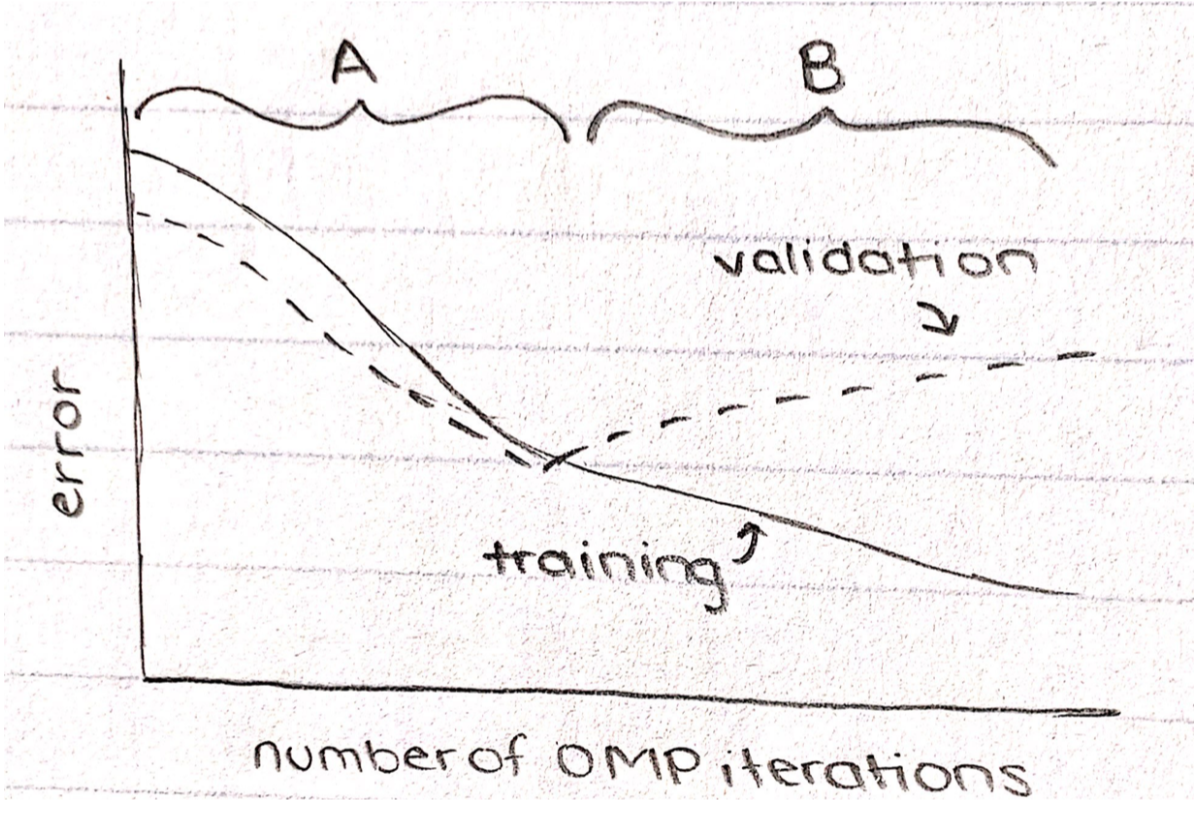
\includegraphics[scale=0.3]{graph}
\end{figure}
    \begin{enumerate}
        \item Region A, Training Error \vspace{2cm}
        \item Region A, Validation Error \vspace{2cm}
        \item Region B, Training Error \vspace{2cm}
        \item Region B, Validation Error \vspace{2cm}
    \end{enumerate}


\end{document}			